
\documentclass[12pt, a4paper]{report}
\usepackage{epsfig}
\usepackage{subfigure}
%\usepackage{amscd}
\usepackage{amssymb}
\usepackage{graphicx}
%\usepackage{amscd}
\usepackage{amssymb}
\usepackage{subfiles}
\usepackage{framed}
\usepackage{subfiles}
\usepackage{amsthm, amsmath}
\usepackage{amsbsy}
\usepackage{framed}
\usepackage[usenames]{color}
\usepackage{listings}
\lstset{% general command to set parameter(s)
	basicstyle=\small, % print whole listing small
	keywordstyle=\color{red}\itshape,
	% underlined bold black keywords
	commentstyle=\color{blue}, % white comments
	stringstyle=\ttfamily, % typewriter type for strings
	showstringspaces=false,
	numbers=left, numberstyle=\tiny, stepnumber=1, numbersep=5pt, %
	frame=shadowbox,
	rulesepcolor=\color{black},
	,columns=fullflexible
} %
%\usepackage[dvips]{graphicx}
\usepackage{natbib}
\bibliographystyle{chicago}
\usepackage{vmargin}
% left top textwidth textheight headheight
% headsep footheight footskip
\setmargins{3.0cm}{2.5cm}{15.5 cm}{22cm}{0.5cm}{0cm}{1cm}{1cm}
\renewcommand{\baselinestretch}{1.5}
\pagenumbering{arabic}
\theoremstyle{plain}
\newtheorem{theorem}{Theorem}[section]
\newtheorem{corollary}[theorem]{Corollary}
\newtheorem{ill}[theorem]{Example}
\newtheorem{lemma}[theorem]{Lemma}
\newtheorem{proposition}[theorem]{Proposition}
\newtheorem{conjecture}[theorem]{Conjecture}
\newtheorem{axiom}{Axiom}
\theoremstyle{definition}
\newtheorem{definition}{Definition}[section]
\newtheorem{notation}{Notation}
\theoremstyle{remark}
\newtheorem{remark}{Remark}[section]
\newtheorem{example}{Example}[section]
\renewcommand{\thenotation}{}
\renewcommand{\thetable}{\thesection.\arabic{table}}
\renewcommand{\thefigure}{\thesection.\arabic{figure}}
\title{Research notes: linear mixed effects models}
\author{ } \date{ }


\begin{document}
	\author{Kevin O'Brien}
	\title{Mixed Models for Method Comparison Studies}
	\tableofcontents
	
\chapter{Appendices}
\section{Appendix 1 : Improper Method Comparison Techniques}
	The issue of whether two measurement methods are comparable to the extent that they can be used interchangeably with sufficient accuracy is encountered frequently in scientific research. Historically, comparison of two methods of measurement was carried
	out by use of paired sample $t-$test, 
	simple linear regression, or correlation coefficients. 
	
	
	\subsection*{Paired sample \emph{t-}test}
	\citet{Bartko} discusses the use of the well known paired sample $t$ test to test for inter-method bias; $H: \mu_{d}=0$. The test
	statistic is distributed as a $t$ random variable with $n-1$ degrees of freedom and is calculated as follows,
	\begin{equation}
	t^{*} = \frac{\bar{d}}{ s_d/\sqrt{n}}
	\end{equation}
	where $\bar{d}$ and $s_{d}$ is the average of the differences of the $n$ observations. This method can be potentially misused for method comparison studies. Paired $t-$tests test only whether the mean responses are the same, and so provides a useful test for inter-method bias. However, no insight can be obtained about the variability of the case-wise differences by the paired $t-$test, critically undermining it as a stand-alone procedure. Only if the two methods show comparable
	precision then the paired sample student $t$-test is appropriate for assessing the magnitude of the bias.
	
	%======================================================================================= %
	
	
	\subsection*{The Correlation Coefficient}
	%----------------------------------------------------------------------------%
	%		\subsection{Pearson's Correlation Coefficient} 
	% %- 			% http://www.jerrydallal.com/LHSP/compare.htm
	
	Correlation is inadequate to assess agreement because it only evaluates only the linear association of two sets of observations.  Nonetheless linear association is not the same as agreement. It is possible for two methods to
	be highly correlated, yet have poor agreement due to any combination of constant and proportional bias. Arguments against its usage have been made repeatedly in the relevant literature,  with \citet{BA83}, \citet{BA86}, \citet{BA2003} and \citet{giavarina2015understanding} as examples.
	%	
	%	
	%		
	%	
	%	The correlation coefficient can be close to 1 even when there is considerable bias between the two methods. For example, if one method gives measurements that are always 10 units higher than the other method, the correlation will be 1 exactly, but the measurements will always be 10 units apart.
	%	
	%	The magnitude of the correlation coefficient is affected by the range of subjects/units studied. 
	%	
	%	The correlation coefficient can be made smaller by measuring samples that are similar to each other and larger by measuring samples that are very different from each other. 
	%	
	
	%----------------------------------------------------------------------------%
	\subsection*{Regression Methods}
	On account of the fact that one set of measurements are linearly related to another, one could surmise that simple linear Regression is the most suitable approach to analyzing comparisons. However simple linear regression  is considered by many authors to be wholly unsuitable for method comparison studies \citep{BA83,CornCoch,ludbrook97}. Simple linear regression is defined as such with the name `Model I regression' by \citet{CornCoch}, in contrast to `Model II regression' models, which shall be discussed later on.
	
	A key assumptions of simple linear regression is that the independent variable values are without random error. 	
	For method comparison studies, both sets of measurement must be assumed to be measured with imprecision and neither case can be taken to be a reference method. Arbitrarily
	selecting either method as the reference (i.e. the independent variable) will yield conflicting outcomes: a regression of $X$ on $Y$ would yield an entirely different model from fitting $Y$ on $X$.
	
	Further criticisms of linear regression exist.
	Firstly regression methods are uninformative about the variability of the differences. Secondly regression models are unduly influenced by outliers. Lastly, regression models can not be used to effectively analyze repeated measurements.	
	
\subsubsection*{The Identity Plot}
	\citet{BA83} states that regression analysis can offer useful insights, and recommending an `Identity Plot', a simple graphical approach that yields a cursory examination of how well the measurement methods agree. In the case of good agreement, the co-variates of the Identity plot accord closely with the $X=Y$ line. This plot is not useful for a thorough examination of the data. \citet{BritHypSoc} notes that data points will tend to cluster around the line of equality,
	obscuring interpretation. An identity plot shall complement demonstrations of commonly used approaches in the next chapter.
	
	
	\subsubsection*{Decomposition of Inter-Method Bias}
	Regression approaches are useful for a making a detailed examination of the biases across the range of measurements, allowing inter-method bias to be decomposed into constant bias and proportional bias. Regression methods can determine the presence of inter-method bias, and the levels of constant bias and proportional bias thereof \cite{ludbrook97,ludbrook02}. 
	
	Constant bias describes the case where one method gives values that are consistently different to the other across the whole range. Using a naive estimation of bias, such as the mean of differences, it may incorrectly indicate absence of bias, by yielding a mean difference close to zero. This would be caused by positive differences in the measurements at one end of the range of measurements being canceled out by negative differences at the other end of the scale. Proportional Bias exists when two methods agree on average, but exhibit differences over a range of measurements, i.e. the differences are proportional to the scale of the measurement.	A measurement method may be subject to any combination of fixed bias or proportional bias, or both \citep{ludbrook02}. 
	
	Constant or proportional bias using linear regression can be detected by an individual test on the intercept or the slope of the line regressed from the results of the two methods to be compared. If there is no constant bias, the intercept is equal to zero and, similarly, if there is no proportional bias, the slope is equal to one. Thus, carrying out hypothesis tests on these coefficients (where the null hypotheses are $\beta_0=0$ and $\beta_1=1$) allow us to test for the presence of both types of bias.
	
	
	If the basic assumptions underlying linear regression are not met, the regression equation, and consequently the estimations of bias are undermined. 
	%Outliers are a source of error in regression estimates.
	

\section{Appendix 2 : Variations of the Bland-Altman Plot} 
The limits of agreement methodology assumes a constant level of bias throughout the range of measurements. As \citet*{BA86} point out this may not be the case. 
Importantly \citet{BA99} makes the following point:
\begin{quote}These estimates are meaningful only if we can assume
	bias and variability are uniform throughout the range of
	measurement, assumptions which can be checked graphically.
	\end{quote}
	
	The importance of this statement is that, should the Bland Altman plot indicate that these assumptions are not met, then their
	entire methodology, as posited thus far, is inappropriate for use
	in a method comparison study. Again, in the context of potential
	outlier in the Grubbs data (figure 1.2), this raises the question
	on how to correctly continue. 
	
	Due to limitations of the conventional difference plot, a series of alternative formulations for the Bland-Altman approach have been proposed. Referring to the assumption that bias and variability are constant across the range of measurements, \citet{BA99} address the case where there is an increase in variability as the magnitude increases. They remark that it is possible to ignore the issue altogether, but the limits of agreement would be wider apart than necessary when just lower magnitude measurements are considered. Conversely the limits would be too narrow should only higher magnitude measurements be used. 
	
	To address the issue, they propose the logarithmic transformation of the data. The plot is then formulated as the difference of paired log values against their mean. Bland and Altman acknowledge that this is not easy to interpret, and may not be suitable in all cases.
	
	\citet{BA99} offers two variations of the Bland-Altman plot that are intended to overcome potential problems that the conventional plot would be inappropriate for. The first variation is a plot of case-wise differences as percentage of averages, and is appropriate when there is an increase in variability of the differences as the magnitude increases. 
	
	The second variation is a plot of case-wise ratios as percentage of averages, removing the need for logarithmic transformation. This approach is useful when there is an increase in variability of the differences as the magnitude of the measurement increases. \citet{Eksborg} proposed such a ratio plot, independently of Bland and Altman. \citet{Dewitte} commented on the reception of this article by saying `\textit{Strange to say, this report has been overlooked}'.
	
	%%%%%%%%%%%%%%%%%%%%%%%%%%%%%%%%%%%%%%%%%%%%%%%
  
  \section{Appendix 3 : The Coefficient of Repeatability}
  
  
  \citet{BA99} strongly recommends the simultaneous estimation of repeatability and agreement by  collecting replicated data. \citet{ARoy2009} notes the lack of convenience in such calculations. The coefficient of repeatability is a measure of how well a measurement method agrees with itself over replicate measurements \citep{BA99}. 
  
  As mentioned previously, \citet{Barnhart} emphasize the importance of repeatability as part of an overall method comparison study. The coefficient of repeatability was proposed by \citet{BA99}, and is referenced in subsequent papers, such as \citet{BXC2008}. \citet{BSIrepeat} define a coefficient of
  repeatability as \emph{the value below which the difference between two single test results....may be expected to lie within a specified probability.} \citet{BA99} defines the repeatability coefficient as the upper limits of a prediction interval for the absolute difference between two measurements by the same method on the same item under identical circumstances. % \citep{BXC2008}.	
  
  Once the within-item variability for both methods has been estimated, the relevant calculations for the coefficients of repeatability are straightforward.
  The coefficient is calculated from the within-item variability $\sigma^2_{m}$ as  $1.96 \times \sqrt{2} \times \sigma_m$ = $2.83 \sigma_m$. For $95\%$ of subjects, two replicated measurement by the same method will be within this repeatability coefficient.
  
  
  The coefficient of repeatability may provide the basis for the formulation a formal definition of a `gold standard'. For example, by determining the ratio of the repeatability coefficient $(CR)$ to the sample mean $\bar{X}$. Advisably the sample size should specified in advance. A gold standard may be defined as the method with the lowest value of $\lambda = CR /\bar{X}$ with $\lambda < 0.1\%$. Similarly, a silver standard may be defined as the method with the lowest value of $\lambda $ with $0.1\% \leq \lambda < 1\%$. Such thresholds are solely for expository purposes.
  
  %------------------------------------------------------------%
  %
  %
  %	
  %\section{Coefficient of Repeatability}
  %The Bland Altman method offers a measurement on the repeatability of the methods. The \emph{Coefficient of Repeatability} (CR) can be calculated as 1.96 (or 2) times the standard deviations of the differences between the two measurements ($d_2$ and $d_1$).		
  %
  %
  %%		
  %%If the standard deviation of a measurement is $\sigma$ the repeatability coefficient is $2\times\sqrt{2} \sigma = 2.83\times \sigma \approx 2.8 \sigma$.
  %%		$\sigma^2_{x}$ is the within-subject variance of method $x$. The repeatability coefficient is $2.77 \sigma_{x}$ (i.e. $1.96 \times \sqrt{2} \sigma_{x}$). 
  %		
  %		The repeatability of measurement methods is calculated
  %		differently under the two models  Under the model assuming
  %		exchangeable replicates (1), the repeatability is based only on
  %		the residual standard deviation, i.e. $2.8\sigma_m$
  %	
  %	
  %	 The coefficient is calculated from the residual standard deviation (i.e. $1.96 \times \sqrt{2} \times \sigma_m$ = $2.83 \sigma_m$).
  
  
  
  
  
  
  
  
  
  
  %The coefficient of repeatability is referenced in subsequent papers, such as \citet{BXC2008} and \citet{ARoy2009}. Furthermore this coefficient features in other branches of measurement analysis. 
  %\textbf{Find Some Papers to back this up}.
  
  %\section{Repeatability in Bland-Altman Blood Data Analysis}
  %
  %The Bland-Altman plot may also be used to assess a method's repeatability by comparing repeated measurements using one single measurement method on a sample of items.
  %
  %The plot can then also be used to check whether the variability or precision of a method is related to the size of the characteristic being measured.
  %
  %Since for the repeated measurements the same method is used, the mean difference should be zero.
  %Therefore the Coefficient of Repeatability (CR) can be calculated as 1.96 (often rounded to 2) times the standard deviation of the case-wise differences.
  %
  %
  % Two readings by the same method will be within $1.96
  %		\sqrt{2} \sigma_w $ or $2.77 \sigma_w $ for 95\% of subjects. This value is called the repeatability coefficient.
  %		
  %		For observer J using the sphygmomanometer $ \sigma_w = \sqrt{37.408} = 6.116$ and so the repeatability coefficient is
  %		$2:77 \times 6.116 = 16:95$ mmHg.
  %		
  %		 For the machine S,$ \sigma_w = \sqrt{83.141} = 9.118$ and the repeatability coefficient is $2:77 \times 9.118 = 25.27$ mmHg.
  
\subsection{Carstensen Coefficient of Repeatability}
	The limits of agreement are not always the only issue of interest, the assessment of method specific repeatability and reproducibility are of interest in their own right. Repeatability can only be assessed when replicate measurements by each method are available.
	
	Under the model for linked replicates, there are two possibilities depending on the circumstances. If the variation between replicates within item can be considered a part of the repeatability it will be $2.8 \sqrt{
		\omega^2 + \sigma^2_m}$.
	
	However, if replicates are taken under substantially
	different circumstances, the variance component $\omega^2$ may be considered irrelevant in the repeatability and one would therefore
	base the repeatability on the measurement errors alone, i.e. use $2.8 \sigma_m$.
	

	
	





\section{Appendix 6 : SEMS and Measurement Error Models}
Several authors, such as \citet{gkelly1985} and \citet{voelkel2005center}, recommend the use of Structural Equation Model from method comparison problems.
Structural equation modelling provides a statistically rigourous analysis, but the approach is undermined in several ways.  Highly complex models can be developed using SEM, but to overcome the problem of identifiability, a large quantity of data must be gathered. Often this is beyond what is practical in the main applications of method comparison studies, namely the medical sciences.  Once simplifications are applied, there is little functional difference between SEM and LMEs.
Furthermore LME models have greater flexibility and can be adapted to any variant of the method comparison research question.


%	\citet{nawarathna2015} Measurement Error Models

\citet{DunnSEME} proposes a measurement error model for use in
method comparison studies. Consider n pairs of measurements
$X_{i}$ and $Y_{i}$ for $i=1,2,...n$.
\begin{equation}
X_{i} = \tau_{i}+\delta_{i}\\
\end{equation}
\begin{equation}
Y_{i} = \alpha +\beta\tau_{i}+\epsilon_{i} \nonumber
\end{equation}

In the above formulation is in the form of a linear structural
relationship, with $\tau_{i}$ and $\beta\tau_{i}$ as the true
values, and $\delta_{i}$ and $\epsilon_{i}$ as the corresponding
measurement errors. In the case where the units of measurement are
the same, then $\beta =1$.

\begin{equation}
E(X_{i}) = \tau_{i}\\
\end{equation}
\begin{equation}
E(Y_{i}) = \alpha +\beta\tau_{i} \nonumber
\end{equation}
\begin{equation}
E(\delta_{i}) = E(\epsilon_{i}) = 0 \nonumber
\end{equation}

The value $\alpha$ is the inter-method bias between the two
methods.

\begin{eqnarray}
z_0 &=& d = 0 \\
z_{n+1} &=& z_n^2+c
\end{eqnarray}

	\subsection{Thompson 1963: Model Formulation and Formal Testing}
	% The standard error of these variance estimates are:
	% \begin{eqnarray}
	% \mbox{var}(\sigma^{2}_{1}) = \frac{2\sigma^{4}_{1}}{n-1} +
	% \frac{\sigma^2_{S}\sigma^2_{1}+\sigma^2_{S}\sigma^2_{2}+\sigma^2_{1}\sigma^2_{2}
	% }{n-1}\\
	% \mbox{var}(\sigma^{2}_{2}) =\quad \frac{2\sigma^{4}_{2}}{n-1} +
	% \frac{\sigma^2_{S}\sigma^2_{1}+\sigma^2_{S}\sigma^2_{2}+\sigma^2_{1}\sigma^2_{2}
	% }{n-1}\nonumber
	% \end{eqnarray}
	
	%For the interval estimates for the variance components,
	%\citet{Thompson} presents three relations that hold simultaneously
	%with probability $1-2\alpha$ where $2\alpha=0.01$ or $0.05$.
	
	%\begin{eqnarray*}
	%|\sigma^2-C_{xy}K| &\leqslant& M(C_{x}C_{y})^{\frac{1}{2}}\\
	%|\sigma^2_{1}-(C_{x}-C_{xy})K|&\leqslant M(C_{x}(C_{x}+C_{y}-2C_{xy}))^{\frac{1}{2}}\nonumber\\
	%|\sigma^2_{2}-(C_{y}-C_{xy})K|&\leqslant
	%M(C_{y}(C_{x}+C_{y}-2C_{xy}))^{\frac{1}{2}}\nonumber
	%\end{eqnarray*}
	
	%\citet{Thompson} contains tables for $K$ and $M$.
	
	\citet{Kinsella} formulates a model for un-replicated observations
	for a method comparison study as a mixed model.
	\begin{eqnarray}
	Y_{ij} =\quad \mu_{j} + S_{i} + \epsilon_{ij} \quad i=1,2...n\quad
	j=1,2\\
	S \sim N(0,\sigma^{2}_{s})\qquad \epsilon_{ij} \sim
	N(0,\sigma^{2}_{j}) \nonumber
	\end{eqnarray}
	
	As with all mixed models, the variance of each observation is the
	sum of all the associated variance components.
	\begin{eqnarray}
	\textrm{var}(Y_{ij}) =\quad \sigma^{2}_{s} + \sigma^{2}_{j} \\
	\textrm{cov}(Y_{i1},Y_{i2})=\quad \sigma^{2}_{s} \nonumber
	\end{eqnarray}
	
	
	The standard error of these variance estimates are:
	\begin{eqnarray}
	\textrm{var}(\sigma^{2}_{1}) =\quad \frac{2\sigma^{4}_{1}}{n-1} +\quad
	\frac{\sigma^2_{S}\sigma^2_{1}+\sigma^2_{S}\sigma^2_{2}+\sigma^2_{1}\sigma^2_{2}
	}{n-1}\\
	\textrm{var}(\sigma^{2}_{2}) =\quad \frac{2\sigma^{4}_{2}}{n-1} +\quad
	\frac{\sigma^2_{S}\sigma^2_{1}+\sigma^2_{S}\sigma^2_{2}+\sigma^2_{1}\sigma^2_{2}
	}{n-1}\nonumber
	\end{eqnarray}
	
	\citet{Kinsella} demonstrates the estimation of the variance terms and relative precisions relevant to a method comparison study, with attendant confidence intervals for both. The measurement model introduced by \citet{Grubbs48,Grubbs73} provides a formal procedure for estimating the variances $\sigma^2$, $\sigma^2_{1}$ and $\sigma^2_{2}$. 
	
	% The standard error of these variance estimates are:
	% \begin{eqnarray}
	% \mbox{var}(\sigma^{2}_{1}) = \frac{2\sigma^{4}_{1}}{n-1} +
	% \frac{\sigma^2_{S}\sigma^2_{1}+\sigma^2_{S}\sigma^2_{2}+\sigma^2_{1}\sigma^2_{2}
	% }{n-1}\\
	% \mbox{var}(\sigma^{2}_{2}) =\quad \frac{2\sigma^{4}_{2}}{n-1} +
	% \frac{\sigma^2_{S}\sigma^2_{1}+\sigma^2_{S}\sigma^2_{2}+\sigma^2_{1}\sigma^2_{2}
	% }{n-1}\nonumber
	% \end{eqnarray}
	
	\citet{kinsella} demonstrates how the Grubbs estimators for the
	error variances can be calculated using the difference values,
	providing a worked example on a data set.
	\begin{eqnarray}
	\hat{\sigma^{2}_{1}}
	\quad=\sum{(y_{i1}-\bar{y{1}})(D_{i}-\bar{D})}\\
	\hat{\sigma^{2}_{2}} \quad=
	\sum{(y_{i2}-\bar{y_{2}})(D_{i}-\bar{D})} \nonumber
	\end{eqnarray}
	
	The value $t$ is the $100(1-\alpha/2)\%$ upper quantile ofStudent's $t$ distribution with $n-2$ degrees of freedom \citep{Kinsella}. The confidence limits for $\Delta_{2}$ are found by substituting $C_{y}$ for $C_{x}$ in (1.2).
	Negative lower limits are replaced by the value $0$. The ratio $\Delta_{2}$
	can be found by interchanging $C_{y}$ and $C_{x}$. A lower confidence limit can be found by calculating the square root. The inequality in equation $1.10$ may also be used for hypothesis testing.
	
	
	where
	
	\begin{eqnarray}
	C_{x}=\quad(n-1)S^2_{x}\nonumber\\
	C_{xy}=\quad(n-1)S_{xy}\nonumber\\
	C_{y}=\quad(n-1)S^2_{y}\nonumber\\
	A=\quad C_{x}\times C_{y} - (C_{xy})^2 \nonumber
	\end{eqnarray}
	
	$t$ is the $100(1-\alpha/2)\%$ quantile of Student's $t$
	distribution with $n-2$ degrees of freedom. $\Delta_{2}$ can be
	found by changing $C_{y}$ for $C_{x}$. A lower confidence limit
	can be found by calculating the square root. This inequality may
	also be used for hypothesis testing.
	
	\citet{Thompson} presents three relations that hold simultaneously
	with probability $1-2\alpha$ where $2\alpha=0.01$ or $0.05$. \citet{Thompson} contains tables for $K$ and $M$.
	
	\begin{eqnarray}
	|\sigma^2-C_{xy}K|\leqslant M(C_{x}C_{y})^{\frac{1}{2}}\\
	|\sigma^2_{1}-(C_{x}-C_{xy})K|\leqslant M(C_{x}(C_{x}+C_{y}-2C_{xy}))^{\frac{1}{2}}\nonumber\\
	|\sigma^2_{2}-(C_{y}-C_{xy})K|\leqslant
	M(C_{y}(C_{x}+C_{y}-2C_{xy}))^{\frac{1}{2}}\nonumber
	\end{eqnarray}	
	
	
	
	
	
	
	


\subsubsection{Estimating the Variance Ratio for Deming Regression}

\begin{eqnarray*}
	x_{i} = \mu +  \beta_{0} + \epsilon_{xi}\\
	y_{i} = \mu +  \beta_{1} + \epsilon_{yi}
\end{eqnarray*}
The inter-method bias is the difference of these biases. In order to determine an estimate for the residual variances, one of the method biases must be assumed to be zero, i.e. $\beta_{0} = 0$. The inter-method bias is now represented by $\beta_{1}$.

\begin{eqnarray*}
	x_{i} &=& \mu + \epsilon_{xi}\\
	y_{i} &=& \mu +  \beta_{1} + \epsilon_{yi}
\end{eqnarray*}

The residuals can be expressed as
\begin{eqnarray*}
	\epsilon_{xi} &=& x_{i} - \mu  \\
	\epsilon_{yi} &=& y_{i} - (\mu + \beta_{1}) 
\end{eqnarray*}

The variance of the residuals are equivalent to the variance of the corresponding observations, $\sigma^{2}_{\epsilon x} =
\sigma^{2}_{x}$ and $\sigma^{2}_{\epsilon y} = \sigma^{2}_{y}$.
\begin{equation}
\lambda = \frac{\sigma^{2}_{yx}}{\sigma^{2}_{y}}.
\end{equation}

Assuming constant standard deviations, and given duplicate measurements, the analytical standard deviations are given by

\begin{eqnarray*}
	SD^{2}_{ax} = \frac{1}{2n} \sum (x_{2i} - x_{1i})^{2}\\
	SD^{2}_{ay} = \frac{1}{2n} \sum (y_{2i} - y_{1i})^{2}\\
\end{eqnarray*}

Using duplicate measurements, one can estimate the analyticalstandard deviations and compute their ratio. This ratio is then used for computing the slope by the Deming method \citep{linnet98}.

\subsection{Using LME models to estimate the ratio (BXC) }
	
	\begin{eqnarray*}
		y_{mi} &=& \mu + \beta_{m} + b_{i} + \epsilon_{mi}\\
	\end{eqnarray*}
with $\beta_{m}$ is a fixed effect for the method $m$ and $b_{i}$ is a random effect associated with patient $i$, and
	$\epsilon_{mi}$ as the measurement error. This is a simple single level LME model. \citet{pb} provides for the implementation of fitting a model. The variance ratio of the residual variances is immediately determinable from the output. 
%This variance ratio can be use to fit a Deming regression, as described in chapter 1.
	
		%============================================================================= %
		
		
\section{Appendix 7: Model II regression}
\citet{CornCoch} argue for the use of methods that based on
the assumption that both methods are imprecisely measured ,and
that yield a fitting that is consistent with both '$X$ on $Y$' and
'$Y$ on $X$' formulations. These methods uses alternatives to the
OLS approach to determine the slope and intercept.

They describe three such alternative methods of regression; Deming, Mandel, and Bartlett regression. Collectively the authors refer to these approaches as Model II regression techniques.

The authors make the distinction between model I and model II regression types.

Model II regression is the appropriate type when the predictor variable “x” is measured with imprecision.

\citet{CornCoch} remark that clinical laboratory measurements usually increase in absolute imprecision when larger values are measured.


In this type of analysis, both of the measurement methods are test methods, with both expected to be subject to error. Deming regression is an approach to model II regression.

Model II regression method also calculates a line of best fit for two sets of data. It differs from Model I regression in that it is derived in a way that factors in for error in the x-axis, as well as the y-axis. \citet{CornCoch} refer to it as 'Model II regression'.		
		
		
\subsection{Ordinary Least Product Regression}
		\citet{ludbrook97} states that the grouping structure can be
		straightforward, but there are more complex data sets that have a hierarchical(nested) model.
		
Observations between groups are independent, but observations
		within each groups are dependent because they belong to the same
		subpopulation. Therefore there are two sources of variation:
		between-group and within-group variance.
		% \vspace{5 mm} \noindent Mean correction is a method of reducing
		%bias.
		%-------------------------------------------------
\subsection{Least Products Regression}
Used as an alternative to Bland-Altman Analysis, this method is also known as `Geometric Mean Regression' and `Reduced Major Axis Regression'. This regression model minimizes the areas of the right triangles formed by the data points' vertical and horizontal deviations from the fitted line and the fitted line.
		
Model II regression analysis caters for cases in which random error is attached to both dependent and independent variables. Comparing methods of measurement is just such a case \citep{ludbrook97, ludbrook02}.
		
Least products regression is the Ludbrookes preferred technique for analysing the Model II case. In this, the sum of the products of the vertical and horizontal deviations of the x,y values from the line is minimized.
		
Least products regression analysis is suitable for calibrating one method against another. It is also a sensitive technique for detecting and distinguishing fixed and proportional bias between
		methods.
		
		Least-products regression can lead to inflated SEEs and estimates that do not tend to their true values an N approaches infinity \citep{draper1998}


\subsection{Classical model for Single Measurements}
\section{Appendix 8: Carstensen's Model}
\citet{BXC2004} presented a simple model to describe a measurement by method $m$, describing the relationship with its real value. The non-replicate case is considered first, as it is the context of the Bland-Altman plots. This model assumes that inter-method bias is the only difference between the two methods.

This model is based on measurements $y_{mi}$ by method $m=1,2$ on item $i = 1,2 \ldots$. We use the term $item$ to denote an individual, subject or sample, to be measured, being randomly sampled from a population

The classical model is based on measurements $y_{mi}$ by method $m=1,2$ on item $i = 1,2 \ldots$
\begin{equation}
y_{mi}  = \alpha_{m} + \mu_{i} + e_{mi}, \qquad  e_{mi} \sim
\mathcal{N}(0,\sigma^{2}_{m}).
\end{equation}
Here $\alpha_m$ is the fixed effect associated with method $m$,
$\mu_i$ is the true value for item $i$ (fixed effect) and $e_{mi}$ is a random effect term for errors.

The random error term for each response is denoted $\varepsilon_{mir}$ having $\mathrm{E}(\varepsilon_{mir})=0$, $\mathrm{Var}(\varepsilon_{mir})=\varphi^2_m$. All the random effects are assumed independent, and that all replicate measurements are assumed to be exchangeable within each method.
\newpage

\subsection{Statistical Model For Replicate Measurements}
Let $y_{Aij}$ and $y_{Bij}$ be the $j$th repeated observations of the variables of interest $A$ and $B$ taken on the $i$th item. The number of repeated measurements for each variable may differ for each item.
Both variables are measured on each time points. Let $n_{i}$ be the number of observations for each variable, hence $2\times n_{i}$ observations in total.

It is assumed that the pair $y_{Aij}$ and $y_{Bij}$ follow a bivariate normal distribution.
\begin{eqnarray}
\left(
\begin{array}{c}
y_{Aij} \\
y_{Bij} \\
\end{array}
\right) \sim \mathcal{N}(
{\mu}, {\Sigma})\mbox{   where } {\mu} = \left(
\begin{array}{c}
\mu_{A} \\
\mu_{B} \\
\end{array}
\right)
\end{eqnarray}
The matrix ${\Sigma}$ represents the variance component matrix between response variables at a given time point $j$.
\begin{equation}
{\Sigma} = \left( \begin{array}{cc}
\sigma^2_{A} & \sigma_{AB} \\
\sigma_{AB} & \sigma^2_{B}\\
\end{array}\right)
\end{equation}
$\sigma^2_{A}$ is the variance of variable $A$, $\sigma^2_{B}$ is the variance of variable $B$ and $\sigma_{AB}$ is the covariance of the two variable. It is assumed that ${\Sigma}$ does not depend on a particular time point, and is the same over all time points.

\newpage
\subsection{Computation (BLUPs)} 
Modern software packages can be used to fit models accordingly. The best linear unbiased predictor (BLUP) for a specific subject $i$ measured with method $m$ has the form $BLUP_{mir} = \hat{\alpha_{m}} + \hat{\beta_{m}}\mu_{i} + c_{mi}$, under the assumption that the $\mu$s are the true item values.


%\citet{BXC2004} describes the above model as a `functional model',
%similar to models described by \citet{Kimura}, but without any
%assumptions on variance ratios. A functional model is . An
%alternative to functional models is structural modelling

\citet{BXC2004} uses the above formula to predict observations for a specific individual $i$ by method $m$;
\begin{equation}BLUP_{mir} = \hat{\alpha_{m}} + \hat{\beta_{m}}\mu_{i} +
c_{mi} 
\end{equation}. 

Under the assumption that the $\mu$s are the true item values, this would be sufficient to estimate parameters. The assumption of exchangeability can be unrealistic in certain situations.
\citet{BXC2004} provides an amended formulation which includes an extra interaction
term $d_{mr} \sim N(0,\omega^{2}_{m}$ to account for this.



Maximum likelihood estimation is used to estimate the parameters.
The REML estimation is not considered since it does not lead to a
joint distribution of the estimates of fixed effects and random
effects parameters, upon which the assessment of agreement is
based.






\subsection{The Fat Data Set}
%
%\subsection{The Fat Data Set}
As an example, \citet{BXC2008} discusses a comparison study of measurements of subcutaneous fat
by two observers at the Steno Diabetes Center, Copenhagen. Measurements are in millimeters
(mm). Each person is measured three times by each observer. The observations are considered to be `true' replicates.

A linear mixed effects model is formulated, and implementation through several software packages is demonstrated.
All of the necessary terms are presented in the computer output. The limits of agreement are therefore,
\begin{equation}
0.0449  \pm 1.96 \times  \sqrt{2 \times 0.0596^2 + 0.0772^2 + 0.0724^2} = (-0.220,  0.309).
\end{equation}


\citet{BXC2008} presents a data set `fat', which is a comparison of measurements of subcutaneous fat by two observers at the Steno Diabetes Center, Copenhagen. Measurements are in millimeters (mm). Each person is measured three times by each observer. The observations are considered to be `true' replicates.
\citet{BXC2008} describes the calculation of the limits of agreement (with the inter-method bias implicit) for both data sets, based on his formulation;

\[\hat{\alpha}_1 - \hat{\alpha}_2 \pm 2\sqrt{2\hat{\tau}^2 +\hat{\sigma}_1^2 +\hat{\sigma}_2^2 }.\]


For the `Fat' data set, the inter-method bias is shown to be $0.045$. The limits of agreement are $(-0.23 , 0.32)$

%For Carstensen's `fat' data, the limits of agreement computed using Roy's
%method are consistent with the estimates given by \citet{BXC2008}; $0.044884  \pm 1.96 \times  0.1373979 = (-0.224,  0.314).$


A linear mixed effects model is formulated, and implementation through several software packages is demonstrated.
All of the necessary terms are presented in the computer output. The limits of agreement are therefore,
\begin{equation}
0.0449  \pm 1.96 \times  \sqrt{2 \times 0.0596^2 + 0.0772^2 + 0.0724^2} = (-0.220,  0.309).
\end{equation}

All of these terms are given or determinable in computer output. The limits of agreement can therefore be evaluated using
\begin{equation}
\bar{y_{A}}-\bar{y_{B}} \pm 1.96 \times \sqrt{ \sigma^2_{A} + \sigma^2_{B}  - 2(\sigma_{AB})}.
\end{equation}



\citet{ARoy2009} has demonstrated a methodology whereby $d^2_{A}$ and $d^2_{B}$ can be estimated separately. Also covariance terms are present in both ${G}$ and ${\Lambda}$. Using ARoy2009's methodology, the variance of the differences is
\begin{equation}
\mbox{var} (y_{iA}-y_{iB})= d^2_{A} + \lambda^2_{B} + d^2_{A} + \lambda^2_{B} - 2(d_{AB} + \lambda_{AB})
\end{equation}
\subsection{RV-IV}
\textbf{\textit{Remark: what paper is this from?}}
For the the RV-IC comparison, $\hat{D}$ is given by
	
\begin{equation}
	\hat{G}= \left[ \begin{array}{cc}
	1.6323 & 1.1427  \\
	1.1427 & 1.4498 \\
	\end{array} \right]
	\end{equation}
The estimate for the within-subject variance covariance matrix is
	given by
	\begin{equation}
	\hat{\Sigma}= \left[ \begin{array}{cc}
	0.1072 & 0.0372  \\
	0.0372 & 0.1379  \\
	\end{array}\right]
	\end{equation}
The estimated overall variance covariance matrix for the the 'RV
	vs IC' comparison is given by
	\begin{equation}
	Block \Omega_{i}= \left[ \begin{array}{cc}
	1.7396 & 1.1799  \\
	1.1799 & 1.5877  \\
	\end{array} \right].
	\end{equation}

\section*{Appendix 10: Liao Shaio}
\citet{LaiShiao} views the uses of linear mixed effects models as an expansion on the Bland-Altman framework, rather than as a replacement.  Their focus is to explain lack of agreement by means of additional covariates outside the scope of the traditional method comparison problem, which extends beyond the conventional method comparison study question. The data used for their examples is unavailable for independent use. 


\section{Appendix 11: Standardization and Studentization} %1.4.2
\newpage
\textit{In this chapter, we will look at residual analysis and diagnostic toold for LME models, and discuss how they can be applied to the method comparison problem.	In classical linear models, a residual is the difference between an observed value and its estimated or predicted value. For LME models, the topic is more complicated, and still a matter of active research. }

\emph{The second part of the chapter looks at diagnostics techniques for LME models, firsly covering the theory, then proceeding to a discussion on 
	implementing these using \texttt{R} code.}

\emph{\citet{schabenberger} describes the examination of model-data agreement as comprising several elements; residual analysis, goodness of fit, collinearity diagnostics and influence analysis.}	
To alleviate the problem caused by inconstant variance, the residuals can be scaled (i.e. divided) by their standard deviations. This results in a \index{standardized residual}`standardized residual'. A random variable is said to be standardized if the difference from its mean is scaled by its standard deviation. The residuals  have mean zero but their variance is unknown, it depends on the true values of $\theta$. Standardization is  not possible in practice. Because true standard deviations are frequently unknown, one can instead divide a residual by the estimated standard deviation to obtain the \index{studentized residual}`studentized residual. 
%Instead, you can compute studentized residuals by dividing a residual by an estimate of its standard deviation. 
If that estimate is independent of the $i-$th observation, the process is termed \index{external studentization}`external studentization'. This is usually accomplished by excluding the $i-$th observation when computing the estimate of its standard error. If the observation contributes to the
standard error computation, the residual is said to be \index{internally studentization}internally studentized.
Externally \index{studentized residual} studentized residual require iterative influence analysis or a profiled residuals variance \textbf{(CITE)}.

To alleviate the problems with the interpretation of conditional residuals that may have unequal variances, we consider sealing.
Residuals obtained in this manner ave called studentized residuals.

\begin{itemize}
	\item Standard residual and influence diagnostics for linear models can be extended to linear mixed models. The dependence of fixed-effects solutions on the covariance parameter estimates has important ramifications in perturbation analysis. 
	\item To gauge the full impact of a set of observations on the analysis, covariance parameters need to be updated, which requires refitting of the model. 
	%	\item The experimental INFLUENCE option of the MODEL statement in the MIXED procedure (SAS 9.1) enables you to perform iterative and noniterative influence analysis for individual observations and sets of observations.
	
	\item The conditional (subject-specific) and marginal (population-averaged) formulations in the linear mixed model enable you to consider conditional residuals that use the estimated BLUPs of the random effects, and marginal residuals which are deviations from the overall mean. 
	\item Residuals using the BLUPs are useful to diagnose whether the random effects components in the model are specified correctly, marginal residuals are useful to diagnose the fixed-effects components. 
	\item Both types of residuals are available in SAS 9.1 as an experimental option of the MODEL statement in the MIXED procedure.
	
	\item It is important to note that influence analyses are performed under the assumption that the chosen model is correct. Changing the model structure can alter the conclusions. Many other variance models have been fit to the data presented in the repeated measures example. You need to see the conclusions about which model component is affected in light of the model being fit.
	%	\item  For example, modeling these data with a random intercept and random slope for each child or an unstructured covariance matrix will affect your conclusions about which children are influential on the analysis and how this influence manifests itself.
\end{itemize}


% \subsubsection{Computation}%1.4.4

The computation of internally studentized residuals relies on the diagonal entries of $\boldsymbol{V} (\hat{\theta})$ - $\boldsymbol{Q} (\hat{\theta})$, where $\boldsymbol{Q} (\hat{\theta})$ is computed as

\[ \boldsymbol{Q} (\hat{\theta}) = \boldsymbol{X} ( \boldsymbol{X}^{\prime}\boldsymbol{Q} (\hat{\theta})^{-1}\boldsymbol{X})\boldsymbol{X}^{-1} \]









\subsubsection{Internally and Externally Studentized Residuals}
%Internally and Externally Studentized Residuals
The computation of internally studentized residuals relies on the diagonal values of $\boldsymbol{V(\hat{\theta})} - \boldsymbol{Q(\hat{\theta})}$
Externally studentized residuals require iterative influece analysis or a profiled residual variance.

Cook's Distance
\[ \boldsymbol{\delta}_{(U)} = \boldsymbol{\hat{\beta}}  - \boldsymbol{\hat{\beta}}_{(U)} \]
A DFFIT measures the change in predicted values due to the removal of data points.
(Belsey, Kuh and Welsch (1980))
%[ \mbox{DFFITS}_{i} = \frac{\hat{y}_i - \hat{y}_{i(U)}}{ese(\hat{y}_i)} \]

$\boldsymbol{D(\beta)}  = \boldsymbol{\delta}^{\prime}_{(U)} \boldsymbol{\delta}_{(U)} / rank(\boldsymbol{X})$
Cook's D can be calibrated according to a chi-square distribution with degress of freedom equal to the rank of $\boldsymbol{X}$ \citep{Christensen}.

%	$ \mbox{CovTrace}(\boldsymbol{\beta})$



\subsubsection{Diagnostic Plots for LME models}





\begin{figure}[h!]
	\centering
	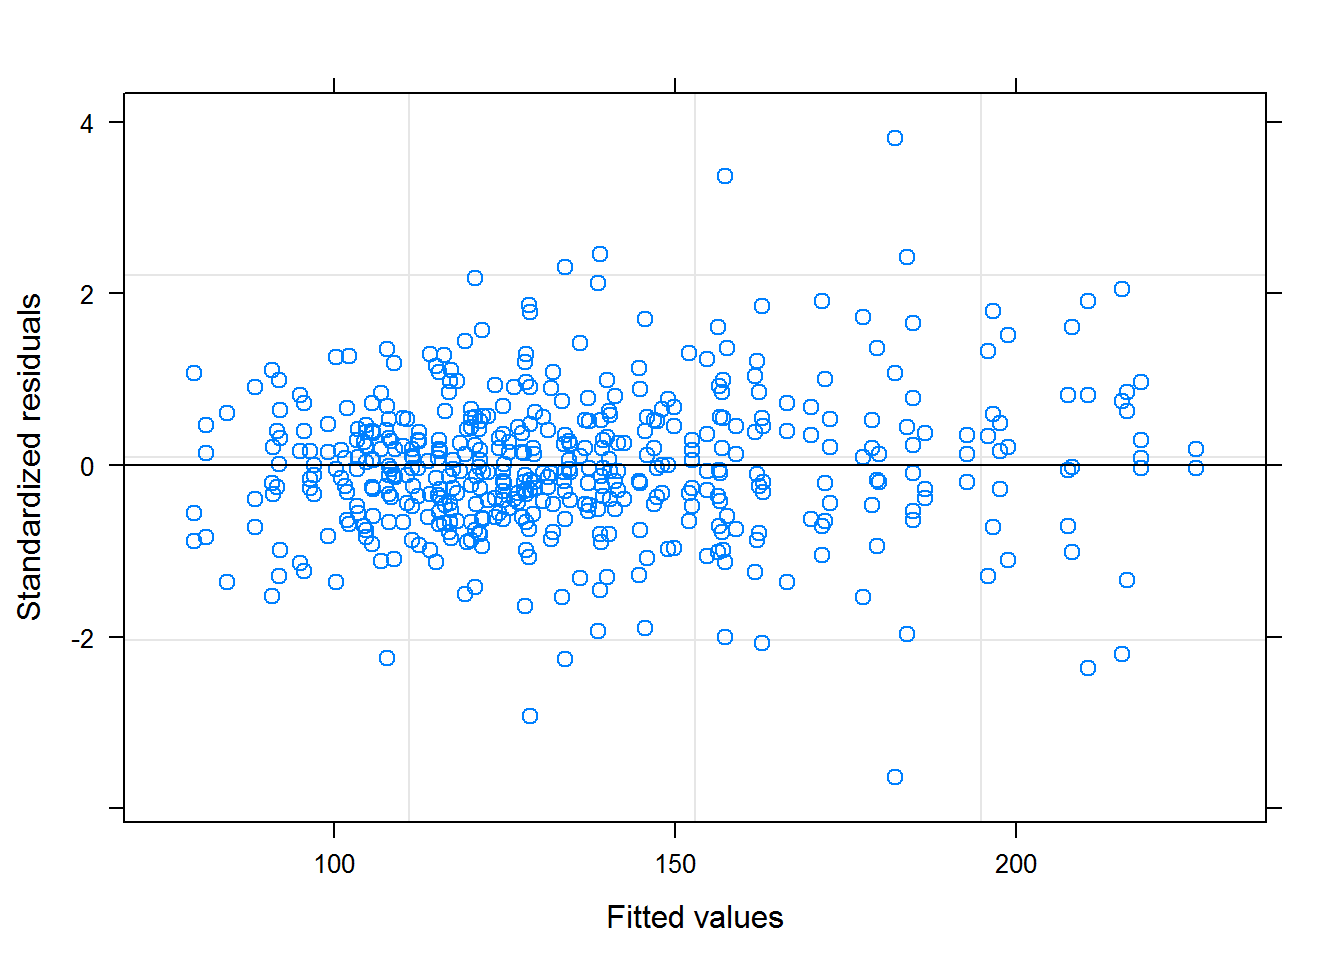
\includegraphics[width=0.9\linewidth]{images/ResidPlot1}
	\caption{}
	\label{fig:ResidPlot1}
\end{figure}



\begin{figure}[h!]
	\centering
	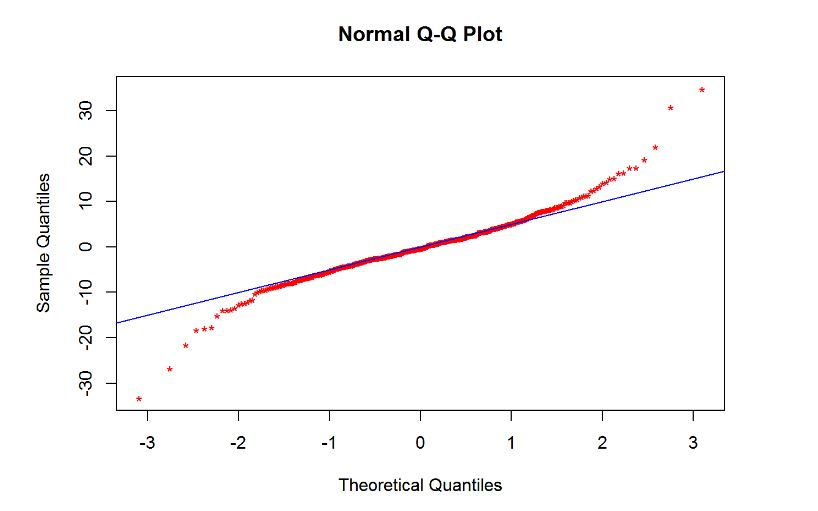
\includegraphics[width=0.7\linewidth]{images/Resid-newplot}
	\caption{}
	\label{fig:Resid-newplot}
\end{figure}




\subsubsection{Reduced Data Set}
It is important to determine if a specific group of cases or subjects give rise to the lack of agreement in the methods. If one were to examine fitted model if these cases were removed.

In this instance, we conclude that there is a systemic diagreement between method S and the other two methods, and that lack of agreement can not be sourced to a handful of cases.
\begin{figure}[h!]
	\centering
	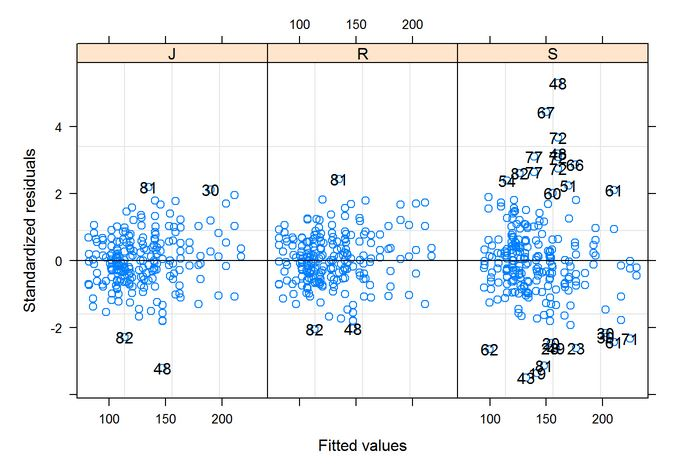
\includegraphics[width=0.7\linewidth]{images/bloodnlmeResidPlot2B}
\end{figure}


\subsubsection{Studentized Residuals}
Standardization is not possible in practice. Studentized residuals are residuals divided by the estimated standard estimation.
[Gregoire,Schabenberger, Barrett (1995)]

\[\boldsymbol{r}_{m} = \boldsymbol{Y} -  \boldsymbol{X} \boldsymbol{\hat{\beta}} \]

\[\boldsymbol{r}_{c} = \boldsymbol{Y} -  \boldsymbol{X} \boldsymbol{\hat{\beta}} -  \boldsymbol{Z} \boldsymbol{\hat{\gamma}}\]

For the individual observation the raw studentized and pearson type residuals are computed as follows:
\[r_{mi} =Y_{i} -X^{\prime} \boldsymbol{\hat{\beta}}\]

\[r_{ci} = r_{mi} - Y_{i} - z_{i}^{\prime} \boldsymbol{\hat{\gamma}}\]











%\subsection{Introduction (Page 1)}
%
%Linear models for uncorrelated data have well established measures to gauge the influence of one or more
%observations on the analysis. For such models, closed-form update expressions allow efficient computations
%without refitting the model. 
%
%
%When similar notions of statistical influence are applied to mixed models,
%things are more complicated. Removing data points affects fixed effects and covariance parameter estimates.
%Update formulas for “\textit{leave-one-out}” estimates typically fail to account for changes in covariance
%parameters. 
%
%Moreover, in repeated measures or longitudinal studies, one is often interested in multivariate
%influence, rather than the impact of isolated points. 

% This paper examines extensions of influence measures
% in linear mixed models and their implementation in the MIXED procedure.









lots of the elements of the marginal residual vector versus the explanatory variables in $X$ can be used to check the linearity of $\boldsymbol{y}$ in a similar manner to the residual plots used in linear models.	Conditional residuals should have mean of zero with no grouping structure. They should be homoscedastic. Conditional residuals are useful for checking normality of outliers

%http://support.sas.com/documentation/cdl/en/statug/63033/HTML/default/viewer.htm#statug_mixed_sect024.htm

In LME models, diagnostic techniques may consider `conditional' residuals. A conditional residual is the difference between an observed value $y_{i}$ and the conditional predicted value $\hat{y}_{i} $.

\[ \hat{\epsilon}_{i} = y_{i} - \hat{y}_{i} = y_{i} - ( X_{i}\hat{\beta} + Z_{i}\hat{b}_{i}) \]

However, using conditional residuals for diagnostics presents difficulties, as they tend to be correlated and their variances may be different for different subgroups, which can lead to erroneous conclusions.
%1.5
%http://support.sas.com/documentation/cdl/en/statug/63033/HTML/default/viewer.htm#statug_mixed_sect024.htm



\section*{Appendix 13: Pearson Residual}%1.4.5
	For an LME model, the \textit{raw} residuals at level $i$ are obtained by subtracting the fitted levels at that level from the response vector If we require a \textit{Pearson} type residual, we further dviide this by the estimated within-group standard error. The Pearson residual is the raw residual divided by the square root of the the within-group standard error for both methods. 
	
	The fitted values at level $i$ are obtained by adding together the population fitted values (based only on the fixed effects estimates) and the estimated contributions of the random effects to the fitted values at grouping levels less or equal to $i$. 
	
	In addition to Raw and Pearson residuals, there are normalized residuals : standardized residuals pre-multiplied by the inverse square-root factor of the estimated error correlation matrix. For the forthcoming examples, we will use the raw residuals.

	
	Another possible scaled residual is the \index{Pearson residual} `Pearson residual', whereby a residual is divided by the standard deviation of the dependent variable. The Pearson residual can be used when the variability of $\hat{\beta}$ is disregarded in the underlying assumptions.
	
	For an \texttt{lme} object, the residuals at level $i$ are obtained by subtracting the fitted levels at that level from the response vector (and dividing by the estimated within-group standard error, if \texttt{type="pearson"}).The Pearson residual is the raw residual divided by the square root of the variance function (here, the Within-group standard error for both methods, 6.11 and 9.11 respectively). The fitted values at level $i$ are obtained by adding together the population fitted values (based only on the fixed effects estimates) and the estimated contributions of the random effects to the fitted values at grouping levels less or equal to $i$.
	
	\begin{description}
		\item[``\texttt{response}"]: the “raw” residuals (\textit{observed - fitted}) are used. This is the default option.
		\item[``\texttt{pearson}"]: the standardized residuals (raw residuals divided by the corresponding standard errors) are used; 
		\item[``\texttt{normalized}"]: the normalized residuals (standardized residuals pre-multiplied by the inverse square-root factor of the estimated error correlation matrix) are used.
	\end{description}


	\section*{Appendix 14 :Conditional and Marginal Residuals}
	
	Suppose the linear mixed-effects model lme has an $n \times p$ fixed-effects design matrix $\boldsymbol{X}$ and an $n \times q$ random-effects design matrix $\boldsymbol{Z}$. 
	
	Also, suppose the p-by-1 estimated fixed-effects vector is $\hat{\beta}$ , and the q-by-1 estimated best linear unbiased predictor (BLUP) 
	vector of random effects is $\hat{b}$ . 
	
	The fitted conditional response is
	
	\[ \hat{y}_{Cond} = X \hat{\beta} + Z \hat{b} \]

	\subsubsection*{Conditional Residuals}
	A conditional probability is the difference between the observed value and the predicted value of the dependent variable.
	\begin{equation*}
	\hat{\epsilon}_{i} = y_{i} - X_{i}\hat{\beta} + Z_{i}\hat{b}_{i}
	\end{equation*}
	
	In general conditional residuals are not well suited for verifying model assumptions and detecting outliers. Even if the true model residuals are uncorrelated and have equal variance, conditional variances will tend to be correlated and their variances may be different for different subgroups of individuals \citep{west}.
	
	%	A conditional residual is the difference between an observed value $y_{i}$ and the conditional predicted value $\hat{y}_{i} $,
	%	\[r_{ci} = y_i - x_i^{\prime} \hat{b} - z_i^{\prime} \hat{\gamma}\]
	%	
	%	\[y - X\beta - Z \eta = \epsilon \]	
	%	
	
	For any type, you can compute the conditional or the marginal residuals. For example, the conditional raw residual is
	
	
	\[ r_{Cond} = y - X \hat{\beta} - Z \hat{b} \]
	
	
	%A conditional residual is the difference between the observed data and the predicted value of the observation,
	%$r_{ci} = y_i - x_i^{\prime} \hat{b} - z_i^{\prime} \hat{\gamma}$
	%
	
	In LME models, diagnostic techniques may consider `conditional' residuals. A conditional residual is the difference between an observed value $y_{i}$ and the conditional predicted value $\hat{y}_{i} $.
	
	\[ \hat{\epsilon}_{i} = y_{i} - \hat{y}_{i} = y_{i} - ( X_{i}\hat{\beta} + Z_{i}\hat{b}_{i}) \]
	
	However, using conditional residuals for diagnostics presents difficulties, as they tend to be correlated and their variances may be different for different subgroups, which can lead to erroneous conclusions.
	
	
	


	\subsubsection*{Marginal Residuals}
	A marginal residual is the difference between the observed data and the estimated (marginal) mean, 
	\[r_{mi} = y_i - x_0^{\prime} \hat{b} =x^{T}_{i}\hat{\beta}\]
	
	\[y - X\beta = Z \eta +\epsilon \]
	
	
	The marginal residuals are defined according to
	\begin{eqnarray*}
		\hat{\xi} = y - X\hat{\beta} = M^{-1}Qy. \\\nonumber
	\end{eqnarray*}
	
	A marginal residual is the difference between the observed data and the estimated (marginal) mean, $r_{mi} = y_i - x_0^{\prime} \hat{b}$. 
	the fitted marginal response is
	
	
	\[ \hat{y}_{Mar} = X \hat{\beta} \]

\section*{Appendix 15: DFFITS}%1.4.5
DFFITS is a diagnostic meant to show how influential a point is in a statistical regression. It is defined as the change, in the predicted value for a point, obtained when that point is left out of the regression, divided by the estimated standard deviation of the fit at that point.	


\bibliographystyle{chicago}
\bibliography{2017bib}
\end{document}	
	
	
	
	
		
		
		
		
				
